% --------------------------------------------------------------------------- %
% Author:          Joey Dumont                <joey.dumont@gmail.com>         %
% Date:            Nov 12th, 2015                                             %
% Description:     Prepared for IHPCSS 2015.                                  %
%                  TikZ code that generates the scattering system used for the%
%                  Stratton-Chu derivation.                                   %
% License:         CC0                                                        %
%                  <https://creativecommons.org/publicdomain/zero/1.0>        %
% --------------------------------------------------------------------------- %

\documentclass[tikz]{standalone}
\usepackage[charted]{mathdesign}
\usetikzlibrary{calc,patterns,decorations.pathmorphing,decorations.pathreplacing,decorations.markings}

\newcommand\irregularcircle[2]{% radius, irregularity
  \pgfextra {\pgfmathsetmacro\len{(#1)+rand*(#2)}}
  +(0:\len pt)
  \foreach \a in {10,20,...,350}{
    \pgfextra {\pgfmathsetmacro\len{(#1)+rand*(#2)}}
    -- +(\a:\len pt)
  } -- cycle
}

\tikzset{
    interface/.style={
        % The border decoration is a path replacing decorator.
        % For the interface style we want to draw the original path.
        % The postaction option is therefore used to ensure that the
        % border decoration is drawn *after* the original path.
        postaction={draw,decorate,decoration={border,angle=45,
                    amplitude=1mm,segment length=1.25mm}}}
}

\begin{document}

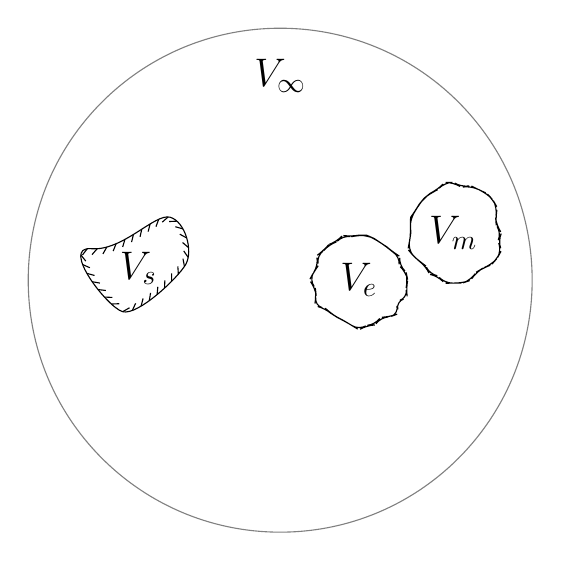
\begin{tikzpicture}[scale=0.20]

   \draw [yshift=-2cm,interface] (0, 0) 
  .. controls ++(165:-1) and ++(240: 1) .. ( 4, 3)
  .. controls ++(240:-1) and ++(165:-1) .. ( 3, 6)
  .. controls ++(165: 1) and ++(175:-2) .. (-2, 4)
  .. controls ++(175: 2) and ++(165: 1) .. ( 0, 0);
  \draw[smooth,rounded corners=1mm] (15,0) \irregularcircle{3cm}{3mm};
  \draw[smooth,rounded corners=1mm] (21,3) \irregularcircle{3cm}{3mm};
  \draw[gray] (10, 0) circle (16);

  \node at (1,0.75) {\Large $V_s$};
  \node at (15,0) {\Large $V_e$};
  \node at (21,3) {\Large $V_m$};

  \node at (10, 13) {\Large $V_\infty$};


\end{tikzpicture}

\end{document}
